\section{SIEM-Systeme}

\label{sec_state_siem}

\begin{itemize}
  \item Was gibt es evtl. gerade im Bereich der Insider-Angriffe schon?
  \item Was ist OSSIM und wie sieht die Architektur aus?
\end{itemize}


Was steht hier so?


\subsection*{OSSIM}

Eine quelloffene SIEM-Lösung, die im Rahmen dieser Arbeit genutzt werden wird, ist OSSIM, ein SIEM-System der Firma AlienVault, das auf Basis weiterer quelloffener Lösungen aus dem Netzwerksicherheits-Bereich unter anderem die in Abschnitt \ref{sec_basics_siem} beschriebenen Funktionen bereitstellt.\footnote{
	AlienVault OSSIM: The World’s Most Widely Used Open Source SIEM\\https://www.alienvault.com/products/ossim
}

\begin{figure}[]
    \centering
        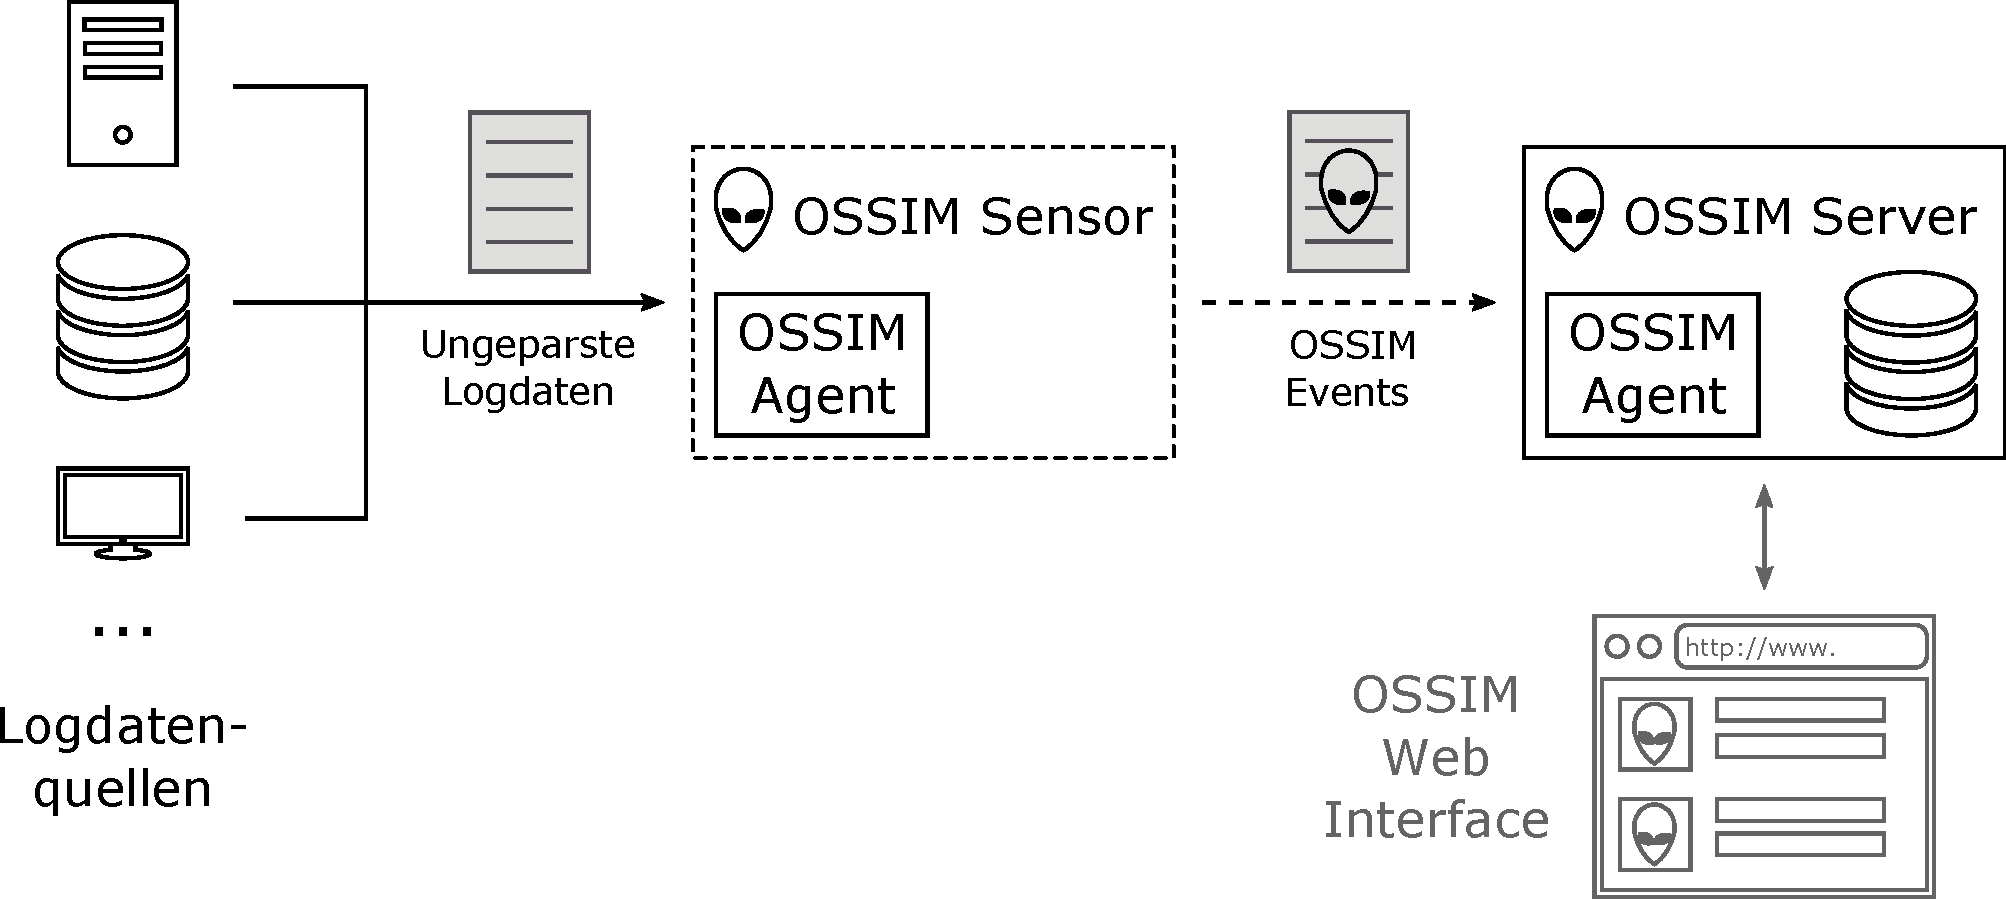
\includegraphics[width=0.9\textwidth]{dia/ossim_log_flow.pdf}
    \caption{High-Level-Übersicht über die OSSIM-Architektur und den Datenfluss.}
    \label{fig:ossim_log_flow}
\end{figure}

- Integrierte Lsg oder externe Sensoren
- Event-Parsing durch Agent mit Plugins (wieviel Details?)
- Bild vom Frontend?
- 